\chapter{相关工作及问题定义}
\label{cha:related}

\section{相关研究工作}
\subsection{安全云存储方案}
可验证的云存储服务已经被广泛的研究过,例如,数据拥有性证明 (Proof of Data Possession, PDP)~\cite{ateniese2007provable, ateniese2008scalable, erway2015dynamic,zhu2012cooperative},数据可取回证明 (Proof of Retrievability, POR)~\cite{juels2007pors, bowers2009proofs, stefanov2012iris} 等等。这些方案主要侧重于云端存储数据的完整性验证,并支持丢失数据的恢复。注意,这些方案与加密搜索场景下的结果验证是不同的,因为加密搜索的结果验证不仅需要验证某个文件本身的完整性,还需要验证整个搜索结果集合是否完整。而这些方案只能单纯验证数据块的完整性,不支持对搜索结果完整性的验证。

\subsection{安全加密搜索方案}
加密搜索的概念首次由Song等人~\cite{song2000practical}在2000年提出,他们的方案允许用户将加密后的数据集存储到云端,并同时保证用户在该加密数据集上进行搜索的能力。随后,加密搜索方案被广泛的研究,总体来说可以分为以下两个分支:对称加密搜索 (Searchable Symmetric Encryption, SSE)和公钥加密搜索 (Public Key Encryption with Keyword Search, PEKS)。其中,最经典的对称加密搜索方案~\cite{curtmola2011searchable}由Curtmola等人提出,他们的方案利用了明文搜索中的倒排索引的思想,并且他们对加密搜索的安全性进行了严格的定义,提出加密搜索方案至少要在面对一个被动敌手的情况下是安全可靠的。目前还有许多不同的对称加密搜索方案实现了不同的搜索功能。例如,动态对称加密搜索 (Dynamic SSE) 方案~\cite{kamara2012dynamic,cash2014dynamic,stefanov2014practical}允许用户更新其数据集, 支持关键字排序 (Ranked Keyword Search) 的对称加密搜索方案~\cite{wang2010secure}允许用户获取根据某一影响因子排序后的搜索结果。最经典的公钥加密搜索方案~\cite{boneh2004public}由Boneh等人提出,他们的方案利用了双线性映射技术。总体来说,公钥加密搜索方案的性能是远远低于对称加密搜索方案的。


\subsection{可验证数据结构}
可验证数据结构 (Authenticated data structure) 在不可信的云存储环境中,主要被用于验证数据块的完整性。典型的可验证数据结构包括:默克尔树 (Merkle Tree, MT)~\cite{merkle1987digital}, 可验证哈希表( Authenticated Hash Table, AHT)~\cite{papamanthou2008authenticated} 以及可验证跳表 (Authenticated Skip List, ASL)~\cite{pugh1990skip,goodrich2001implementation}。其中,默克尔树是最常见的用于验证数据完整性的数据结构,但是默克尔树对数据更新的支持不够灵活。采用默克尔树实现的可验证对称加密搜索方案~\cite{kamara2011cs2}由于没法在中间节点存储关键字信息,因此也不支持与关键字相关的搜索。可验证哈希表采用了RSA累加器~\footnote{RSA为提出该算法的三个密码学家名字的首字母,分别为Ron Rivest, Adi Shamir, 和Leonard Adleman} (RSA Accumulator) 方法来实现数据验证,但是它的搜索和更新性能都较低。具体而言,可验证哈希表的搜索与更新速度在毫秒级别,而我们采用的默克尔帕特里夏树的搜索更新速度在微秒级别。可验证跳表采用了类似多级链表的方式来实现,一定程度上提升了搜索性能,但如果它将关键字信息存储于搜索路径上,存储空间将比默克尔帕特里夏树大很多。


\subsection{可验证对称加密搜索方案}
由Kamara等人提出的CS2方案~\cite{kamara2011cs2}通过使用默克尔树构建验证索引来支持用户对搜索结果的验证。具体的做法是,以加密的关键字作为“键”,以该关键字对应的加密文件集合作为“值”,将该“键值对”存储在默克尔树的叶子结点上。用户在本地需要保留默克尔树的根哈希作为一个指纹信息。在进行结果验证时,用户需要通过其搜索的关键字本身及服务器返回的该关键字对应在默克尔树上的路径来重构出该根哈希,并与保留的根哈希进行比对,从而来进行结果验证。但是他们的方案无法检测服务器恶意返回空结果的情况。关键的原因是,当用户搜索的关键字不存在时,默克尔树上不会存在该关键字对应的路径,因此服务器无法返回任何信息给用户。解决该问题的一个简单的方法是在构建默克尔树时,将整个字典空间中所有可能的关键字集合都存储在默克尔树中,但这样做会导致大量的空间浪费。

近期,Kurosawa等人提出了一系列可验证对称加密搜索方案~\cite{kurosawa2012uc,kurosawa2013update,ogataefficient}。但是他们的方案要么效率很低,要么不支持用户数据动态更新。其中方案~\cite{kurosawa2012uc}需要线性搜索时间并且不支持数据动态更新。他们的扩展方案~\cite{kurosawa2013update}支持了用户数据更新,该方案通过消息验证码 (Message Authenticated Code, MAC)来确保了数据完整性,通过RSA累计器确保了数据新鲜性,但是方案的搜索复杂度超过了线性时间,并且该方案需要用户在本地维护一个关键字集合来探测服务器故意返回空结果的情况,这将引入较大的空间开销。Ogata等人也提出了一个通用的可验证对称加密搜索框架~\cite{ogataefficient},该方案可以为任何对称加密搜索方案提供结果验证服务,并且不需要用户自己在本地维护一个关键字集合,但是他们的方案仍然是一个静态的方案,即不支持用户数据更新。方案~\cite{chai2012verifiable} \cite{cheng2015verifiable}也同样只是静态方案。

由Stefanov等人提出的方案~\cite{stefanov2014practical}采用了时间戳和消息验证码机制来实现了结果验证,但是他们的方案没法防御服务器故意返回空结果来规避结果验证的情况。Bost等人提出的方案~\cite{bost2016verifiable}是目前为止最完善的普适性可验证对称加密搜索方案,但他们的方案在搜索时需要与服务器进行两轮通信,加密搜索和结果验证过程在服务器端无法并行进行,即用户需要在拿到加密搜索的结果后再与服务器进行通信来进行验证,这将导致较大的验证时延和通信开销,并且他们的方案同样也不支持多用户情况下的验证。

总体来说,一个完善的普适性可验证对称加密搜索方案首先应该支持数据新鲜性和数据完整性验证,尤其要关注搜索结果为空时的验证,这一点被大部分的方案忽略。
其次该方案应该在支持结果验证的同时,尽量降低用户本身的存储和计算开销,例如不需要用户本身去维护一个本地关键字集合。
另外,该方案还应该支持用户数据的更新,并且能够支持多用户场景下的结果验证。
综上所述,在单用户场景中,现有的可验证加密搜索方案无法在保证验证效率的同时,完善地验证数据新鲜性和数据完整性。并且现有的方案都不能满足多用户场景下的对称加密搜索结果验证。这需要我们利用合理的数据结构,并设计合理的机制来设计一个普适的可验证对称加密搜索框架。

\subsection{可验证公钥加密搜索方案}
第一个可验证的非对称加密搜索方案~\cite{zheng2014vabks}由Zheng等人提出,他们的方案采用了基于属性的关键字(Attribute-based keyword,ABK),但是他们的方案也只适用于数据库静态的情况。基于他们的工作,Liu等人又提出了一个更高效的可验证非对称加密搜索方案~\cite{liu2014efficient},Sun等人也提出了一个支持多关键字搜索的可验证公钥加密搜索方案~\cite{sun2015catch}。然而,由于非对称加密本身的限制,他们的方案必不可少地需要引入一个可信第三方,并且搜索的性能大大低于可验证对称加密搜索方案。

\subsection{多用户加密搜索方案}
目前有一些多用户场景下的加密搜索方案~\cite{curtmola2011searchable,yang2009multiuser,jarecki2013outsourced,sun2016efficient},但这些方案都不支持结果验证。Curtmola等人在2006年即提出了一个基于广播加密的多用户加密搜索方案~\cite{curtmola2011searchable},该方案允许数据持有者将数据分享给其他用户,并且数据持有者可以设定其他用户的访问控制权限,可以随时撤销或者新增用户。Yang等人也通过双线性映射 (Bilinear Mapping) 技术提出了一种支持多用户读多用户写的方案~\cite{yang2009multiuser},但是该方案的搜索效率与数据集合的大小成正比,无法应用于数据量很大的场景中。Jerecki等人随后又提出了一个多用户加密搜索方案~\cite{jarecki2013outsourced},然而该方案需要数据持有者和搜索用户进行频繁的交互,给数据持有者带来了很大的通信开销。近期,Sun等人提出了一个非交互式的多用户加密搜索方案~\cite{sun2016efficient},该方案降低了数据持有者的通信开销,但他们的方案不支持用户数据更新。注意,这里我们需要强调,下文我们提出的多用户场景下的可验证对称加密搜索方案旨在为实现了多用户加密搜索的方案提供一个跨用户的结果验证,而不是旨在设计一个多用户方案。据我们目前所知,现有的可验证对称加密搜索方案都只支持单用户场景下的结果验证,而不支持多用户场景下的结果验证,因为多用户场景下的结果验证会面临更多的困难。例如,当数据在不同用户之间共享时,由于数据搜索用户无法探知数据持有者是否对数据集合进行了更新,因此一个恶意的服务器可以返回旧数据集合的搜索结果。除非数据持有者在每次更新时都通知所有的搜索用户,但这将会带来很大的通信开销。我们将在第~\ref{cha:multi-user} 章具体讲述我们的多用户方案。

\section{先验知识}

\subsection{增量哈希}
增量哈希 (Incremental Hash, IH) 由Bellare等人提出~\cite{bellare1994incremental},并被已有的加密搜索方案~\cite{kamara2011cs2}所使用。增量哈希函数是一个抗碰撞的函数:$IH: \{0,1\}^* \rightarrow \{0,1\}^l$,两个随机字符串通过增量哈希函数相加或相减后,生成的哈希值不会产生碰撞。举例来说,假设 $D$ 是一个包含关键字 $w$ 的数据集合,它的增量哈希值为 $H$。 当一个新数据 $d$ 加入到 $D$ 中后, 新的数据集合变为 $D'$ ,即 $D+d$。对于原有数据集 $D$ 来说,数据 $d$ 的加入只是微小的变动。这使得增量哈希函数可以基于数据 $d$ 和现有哈希值 $H$,并通过“加法”操作快速的计算出新文件集 $D'$ 的一个抗碰撞哈希值,而不需要基于新文件集 $D'$ 重新计算哈希值,这使得哈希操作的性能得到了较大的提升。
 %Incremental hash was proposed by Bellare et al.~\cite{bellare1994incremental} and was used by existing SSE schemes, e.g., CS2~\cite{kamara2011cs2}. An incremental hash function is a collision-resistant function $IH: \{0,1\}^* \rightarrow \{0,1\}^l$, with which the addition or the subtraction operation of two random strings on the $IH$ does not produce a collision. For example, assuming $F$ is a file collection that contains the keyword $k$. After a new file $f$ is inserted to $F$, the file collection becomes $F'$ (i.e., $F+f$), which means the new file $f$ is a slight change according to $F$.  Therefore, an incremental hash function can be used to quickly compute the corresponding collision-resist hash value after a file change. More detailed descriptions can be found in~\cite{kamara2011cs2}.


%【IH】Thank the reviewer for pointing out this issue. We reviewed the incremental hash in Section 2. An incremental hash function is a collision-resistant function, which was first proposed by Bellare et al. [22]. We revised the description of the incremental hash in Section 2.
%In our scheme, if a file collection of a data owner is changed, the data owner uses the incremental hash function to quickly calculate a collision-resistance hash value of the changed data, which achieves high efficiency in computing hash values. Another advantage is that, when a file is added or deleted, a collision-resistance hash value ensures the security of our scheme during update.
\subsection{默克尔帕特里夏树}
默克尔帕特里夏树 (Merkle Patricia Tree, MPT) 最早在以太坊~ \cite{wood2014ethereum, merkle_patricia_tree} (Ethereum) 中提出,它将传统的字典树 (Trie Tree) 和默克尔树结合,使得该树同时具有查找和验证的功能。MPT具有四种类型的节点,分别为空节点(Blank Node,BN),叶子节点(Leaf Node,LN),分支节点(Branch Node,BN)和扩展节点(Extension Node,EN)。其中空节点只是一个不存任何信息的节点,叶子节点存储了键值对(key-value pair),扩展节点也存储了键值对,但扩展节点的键值分别为其子节点的公共前缀和子节点的哈希值。分支节点有17个元素,其中前16个元素代表了该节点上有可能的分支,即16个十六进制数字,第17个元素为值。当某一个关键字在该分支节点匹配完成时,该关键字对应的值就存储该元素中。

\begin{figure}[t]
\centering
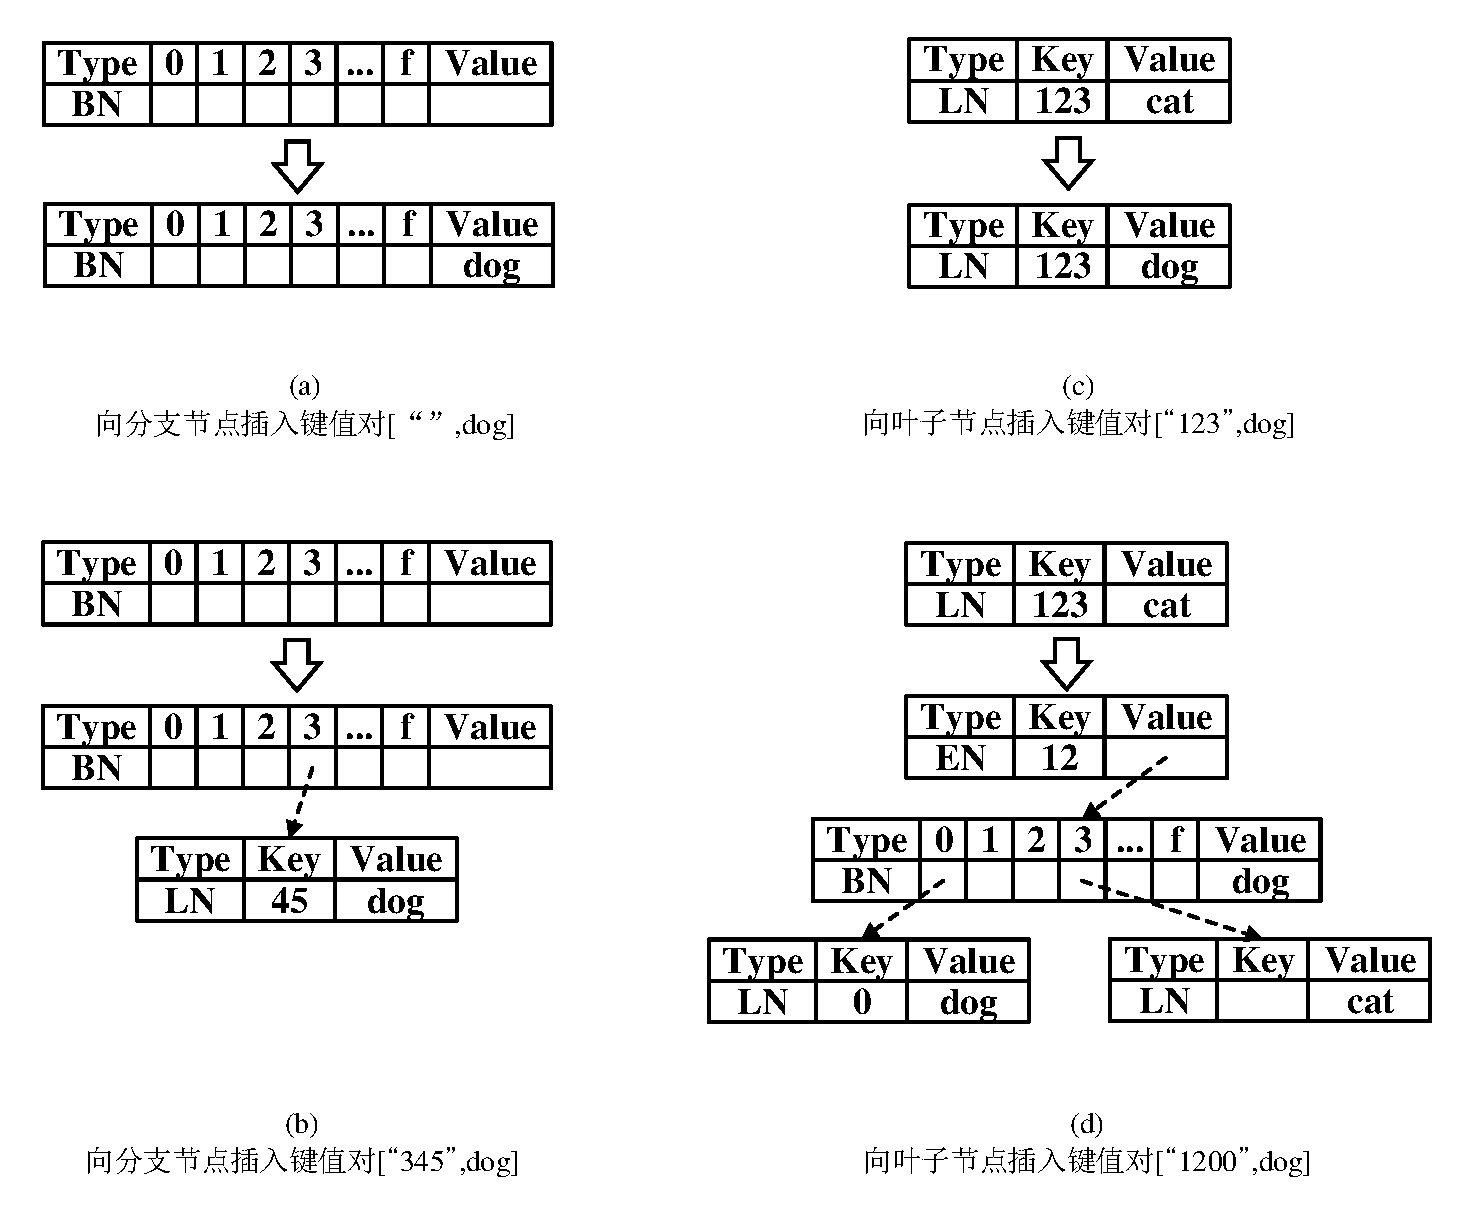
\includegraphics[width=6 in]{fig/MPTUpdate}
\DeclareGraphicsExtensions.
\caption{The Merkle Patricia Tree}
\label{fig:MPTUpdate}
\end{figure}

图~\ref{fig:MPTUpdate} 通过四个简单的例子展示了MPT树的插入过程。首先是将一个“键值对”插入到分支节点,这分为两种情况。如果当前的键空间已经为空,我们可以直接将“值”插入到分支节点的第17个位置。否则,在经过了分支节点匹配后,键空间中“剩余键”和“值”将会存储在分支节点指向的一个新的叶子节点中。其次是将“键值对”插入到叶子节点,也分为两种情况。如果当前键空间中“剩余键”与叶子节点中的“键”正好匹配,直接将叶子节点中的“值”修改为新的“值”即可。否则,我们将找到当前键空间“剩余键”和叶子节点“键”的共同前缀,将其作为一个新建的扩展节点的“键”,并新建一个分支节点,将现有的叶子节点和新建的叶子节点作为子节点插入到分支节点对应的空间中。

注意,MPT中的每一个节点都通过可递归长度前缀法~\cite{RLP_code}(Recursive Length Prefix, RLP) 进行了编码并对编码值再进行了哈希。数据库中存储了每个节点的“键值对”键值对,其中“键”为该节点RLP编码的哈希,“值”为该节点的RLP编码。这样每个节点可以通过他的哈希值被引用,同时保证了MPT的可搜索性和可验证性。通过这种方式,MPT的根哈希成为了整棵树的指纹信息,根哈希的值由所有下层节点的哈希值所决定,任何节点的微小改变都会导致根哈希的值发生变化。此外,MPT与默克尔树不同,MPT是完全确定性的,即一组相同的“键值对”采用不同的顺序插入到MPT中,最终得到的根节点哈希值是相同的,而默克尔树不具有这个性质。
%The Merkle Patricia Tree (MPT) is first proposed in Ethereum~ \cite{wood2014ethereum, merkle_patricia_tree}, which combines the Trie Tree and the Merkle Tree for data update efficiency. There are three kinds of nodes in an MPT to achieve the goal. Leaf Nodes(LN) represents [key,value] pairs. Extension Nodes(EN) represent [key,value] pairs where keys are the public prefixes and their values are the hashes of the next nodes. The Branch Nodes (BN) are used to store possible branches when the prefixes of the keywords differ, which is presented with 17 elements. Among the 17 elements, the first 16 elements represent the 16 possible hex characters in a key and the last element stores a value if a key in a [key,value] pair matches the node.

%Note that, each node of the MPT is represented by its hash and is encoded using Recursive Length Prefix (RLP) code that is mainly used to encode arbitrarily binary data~\cite{RLP_code}, which ensures the cryptographically security of the search operations. The root hash in MPT becomes a fingerprint of the entire tree and is computed based on all hashes of nodes below. Therefore, any modification in a node would incur recomputation of the root hash. Note that, the MPT is fully deterministic, meaning that an MPT with the same [key,value] pairs is exactly the same regardless of the order of insertion, which is different from the Merkle Tree.



%Searchable Encryption was first proposed by Song et al. \cite{song2000practical}, their solution allows a user to outsource its encrypted data to cloud services, and meanwhile retaining the ability to search over it. Normally, searchable encryption has been divided into two categories, i.e.,  Searchable Symmetric Encryption(SSE) and Public Key Encryption with keyword search(PKE). The most classical SSE scheme was proposed by Curtmola et al. in~\cite{curtmola2011searchable}. They defined  privacy against passive adversaries (i.e., honest but curious servers) and developed their scheme by using an inverted index. There exist various SSE schemes with different secure searching functionalities. For example, dynamic SSE schemes~\cite{kamara2012dynamic,cash2014dynamic,stefanov2014practical} allow a user to update his dataset and ranked keyword search scheme~\cite{wang2010secure} that allow a user to retrieve  ranked search results from the server. The most famous PKE scheme was proposed by Boneh et al.~\cite{boneh2004public} with the bilinear map. Normally, the efficiency of the PKE schemes are much lower than the SSE schemes.

%【SSE】Thanks for the suggestions. We explained the secure searchable encryption schemes in Section 2. Searchable encryption allows the server to perform search operations without seeing plaintext data. It empowers the server an ability to search over ciphertext and ensures the security of data on the server. In this revised manuscript, we discussed the existing categories of searchable encryption in Section 2.

\section{问题定义}
在本节中,我们将正式定义方案的攻击模型,方案需要解决的问题以及方案需要实现的目标。

\subsection{攻击模型}
在单用户场景中,数据持有者和数据搜索用户是同一人,而在多用户场景中,这两者是分开的。我们假定数据持有者本身是可信的,而数据搜索用户不可信。此外,我们假定提供存储和搜索服务的云服务器是不可信的,即 1) 云服务器会试图从用户的加密数据和搜索请求中推断出一些隐私信息; 2) 云服务器有可能会因为外部攻击、配置错误、软件错误等原因背离原有协议,从而导致产生数据新鲜性攻击和数据完整性攻击,用以节省其自身的计算开销和通信开销。数据新鲜性攻击和数据完整性攻击的正式定义如下:

\begin{definition}[\textbf{数据新鲜性攻击}]\label{def:freshness}
    {\itshape
			在对称加密搜索中,数据新鲜性攻击是指一个恶意的云服务器试图从旧数据集中返回搜索结果,而不从最新的数据集中返回搜索结果。正式地,让$\Delta_{n-1} = \{\delta_1,\delta_2,\cdots,\delta_{n-1}\}$ 代表用户数据集的历史版本, $\delta_n$ 代表用户的最新数据集,云服务器返回的搜索结果为 $\delta_i$ 的子集,其中 $1 \le i \le n-1$。
      %A data freshness attack in SSE is that a malicious server (or an attacker) attempts to return the historical version of the search result, not the most recently updated version. Formally, let $\Delta_{n-1} = \{\delta_1,\delta_2,\cdots,\delta_{n-1}\}$ denote the historical version of the dataset and $\delta_n$ is the latest version. However, the search result returned by the server is retrieved from $\delta_i$ where $1 \le i \le n-1$.
    }
\end{definition}

\begin{definition}[\textbf{数据完整性攻击}]\label{def:integrity}
    {\itshape
			在对称加密搜索中,数据完整性攻击是指一个恶意的云服务器试图篡改搜索结果,阻止数据搜索用户获取到完整的搜索结果。正式地,让 $\tau$ 代表对称加密搜索方案中的搜索令牌,$\delta_i$ 代表数据集,其中 $1 \le i \le n$。对应的搜索结果应为 $\mathcal{F}(\delta_i, \tau)$,但云服务器返回的搜索结果为 $\mathcal{G}(\delta_i, \tau)$, 其中$\mathcal{G}(\delta_i, \tau) \neq \mathcal{F}(\delta_i, \tau)$。
      %A data integrity attack in SSE is that a malicious server (or an attacker) attempts to tamper with the search result to prevent authenticated users from accessing the complete and correct search result. Formally, let $\tau$ be the search token of the SSE scheme, and $\delta_i$ be the dataset, where $1 \le i \le n$, the corresponding search result should be $\mathcal{F}(\delta_i, \tau)$, but the result returned by the server is $\mathcal{G}(\delta_i, \tau)$, where $\mathcal{G}(\delta_i, \tau) \neq \mathcal{F}(\delta_i, \tau)$.
    }
\end{definition}

%We assume that the data owner is trusted and the data users authorized by the data owner are also trusted\footnote{Please refer to Section \ref{Sec:Discussion} for details on how we can enforce such assumption in practice with multi-user access control techniques.}.
%We consider cloud services performing searchable symmetric encryption (SSE) to be untrusted, which means 1) cloud services intends to derive some sensitive information from the encrypted data and the queries; 2) cloud services may deviate from the prescribed protocols and mount a data freshness attack or a data integrity attack to save its computation or communication cost. The definitions of the data freshness attack and the data integrity attack are presented as follow:

%在可验证加密搜索中,由于服务器不诚信导致的安全性攻击主要可以分为以下两种:
%	重放攻击(Replay Attack):在加密搜索中,重放攻击是指服务器(攻击者)试图返回旧的搜索结果,而不是最新的搜索结果。我们用Δ_n={δ_1,δ_2,⋯,δ_n}来表示旧版本的数据集,用δ_(n+1)来表示最新的数据集,则服务器返回的搜索结果是数据集δ_i的搜索结果,其中1≤i≤n。
%	数据完整性攻击(Data Integrity Attack):在加密搜索中,数据完整性攻击是指服务器(攻击者)试图不让用户获取完整的搜索结果。我们用τ来表示加密搜索中用户的搜索陷门,用户应该得到的搜索结果为F(τ),而服务器返回的搜索结果为G(τ),其中G(τ)⊂F(τ)并且G(τ)可能为∅。
%重放攻击仅存在于动态的加密搜索方案中,在数据库静态的情况下不存在。但现实中,动态数据库较为常见,因此重放攻击是可验证加密搜索必须要解决的问题。数据完整性攻击不仅包括服务器少返回搜索结果的情况还包括了服务器不返回搜索结果来规避结果验证的情况。


\subsection{设计目标}

本论文旨在设计一种普适的可验证加密搜索框架,即该方案可以和任意加密搜索方案相结合,包括但不限于~\cite{stefanov2014practical,cash2014dynamic,kamara2012dynamic},使其能够完成结果验证的功能。本方案将现有的加密搜索方案当做黑盒,总体来说,需要满足以下几个需求:

\begin{enumerate}
	\item \textbf{机密性:} 数据和关键字的机密性是加密搜索最近本的安全需求。它保证了用户的明文数据和关键字信息无法被其他不可信第三方所推断。并且保证了敌手无法从方案的加密数据集,验证索引以及搜索关键字中推断出任何有用的隐私信息。
	%The confidentiality of data and keywords is the most important privacy requirements in SSE. It ensures that users' plaintext data and keywords cannot be revealed by any unauthorized parties, and an adversary cannot learn any useful information about files and keywords through the proof index and update tokens used in %\name.
	%In our scheme, data privacy and keyword privacy is guaranteed by its underlying cipher. Moreover, the search pattern of our scheme is hiding by trading the space.
	\item \textbf{可验证性:} 一个可验证的对称加密搜索方案应该能够验证搜索结果的正确性和完整性,即防止重放攻击和数据完整性攻击。%A verifiable SSE scheme should be able to verify the freshness and integrity of the search results for users.
	%In our scheme, we design a proof algorithm based on the proof structure to detect the dara integrity attacks and meanwhile use the chained-timestamp mechanism to detect the replay attacks.
	\item \textbf{高效性:} 一个可验证对称加密搜索方案应该达到次线性的计算复杂度,即对数复杂度 $O(log(|W|))$,其中 $|W|$ 是关键字的总数,并且应该在支持用户数据更新的情况下仍然能达到该复杂度。注意,这里的计算复杂度仅仅指服务器提供结果验证服务时所需的额外计算复杂度,不包括加密搜索方案本身带来的计算复杂度。%A verifiable SSE scheme should achieve sublinear computational complexity, e.g. logarithmic $O(log(|W|))$, where $|W|$ is the number of keywords, even with file update. Note that, the computational complexity only refers to the cost of searching operations for verification, which does not include the complexity of the searching operations in the existing SSE schemes.
	%Update efficiency, search efficiency and verification efficiency is the most improtant indicator we aim to achieve. In our scheme, we leverage the Mekle Patricia Tree (MPT) which provides the $O(log(n))$ efficiency for search and update which is the optimal solution to the best of our knowledge.
\end{enumerate}

	%机密性:数据和关键字机密性是加密搜索中最重要的隐私需求。其中,数据机密性要求用户的明文数据不能被云服务器获取,关键字机密性要求关键字和文件的相关性不能被云服务器所推断。
	%可验证性:一个可验证的加密搜索方案应该能够验证搜索结果的正确性和完整性,即防止重放攻击和数据完整性攻击。
	%效率:一个可验证的加密搜索方案应该在搜索和更新时具有合理的计算复杂度,例如O(log⁡(|W|)),其中|W|是关键字的数目。


  %This paper aims to provide result verification for any SSE schemes, including but not limited to~\cite{stefanov2014practical,cash2014dynamic,kamara2012dynamic}. Therefore, we treat an existing SSE scheme as a black box such that our proposed scheme can be applied to these SSE schemes for result verification.
